\subsection{Automata}

We use both non-deterministic and deterministic automata 
to convert regex to a lexer. 

Every regex expression has a non-deterministic finite 
automaton that matches, and a deterministic finite 
automaton (DFA) can be algorithmically made from any 
NFA according to the rules in Figure \ref{fig:nfa2dfa}.
\begin{figure}
    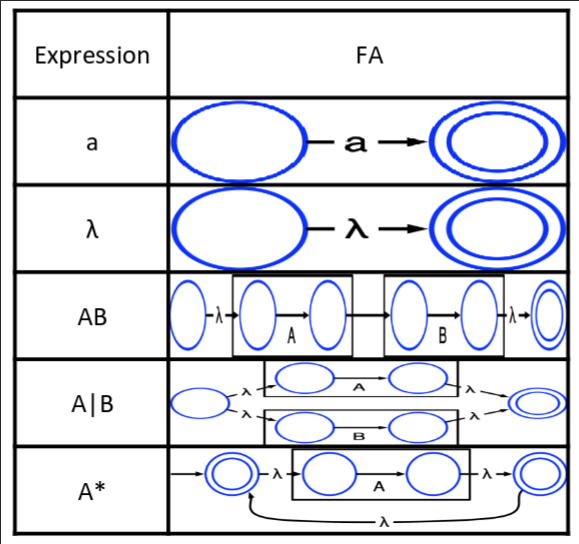
\includegraphics{images/nfa_dfa_conversion.png}
    \caption{NFA to DFA Conversion Rules}
    \label{fig:nfa2dfa}
\end{figure}
% idk why this reference doesn't work and 
% like half the class went by before i gave up
The DFA built from an NFA according to these rules
is not necessarily optimized, so it should be 
minimized using transition partiitioning. Two states 
are equivalent if they have the same accepting/not accepting 
status and if they have the same transitions for a given 
input. If state $A$ and $B$ are both accepting and 
both move to state $C$ on input $a$, then they are 
the same state. Keep merging states according to these 
rules until there are no changes to get the minimized 
DFA. 